


Throughout this assignment, let $G = (V,E)$ be a connected graph
and $w: E \rightarrow \R^+$ be a weight function.\\

\begin{exercise}
    Prove the inverse of the cut lemma:
      If $X$ is good, $e \not \in X$, and $X \cup e$ is good,
      then there is a cut $S, V\setminus S$ such that (i) no
      edge from $X$ crosses this cut and (ii) $e$ is a minimum
      weight edge of $G$ crossing this cut.
\end{exercise}
\begin{proof}
    Since $X \cup \{e\}$ is good, let $\{e\}\in T$, and $T$ is a minimum spanning tree. Delete $e$ in $T$ and then we will get two connected components. Let $S$ be the set of vertices in one connected component.

    (i) Because obviously $X\subset T$, and $e$ is the only element that crosses the cut, $X$ has no edge that crosses the cut.

    (ii) Assume there exists an edge $e'$ with a smaller weight than $e$. Because it is not chosen when forming the spanning tree, it must form a cycle in $S$ or $V\setminus S$. Otherwise, at that step of considering $e'$, $e$ has not been in the spanning tree, and then $e'$ cannot form a cycle across the cut.
\end{proof}

\begin{definition}
  For $c \in \R$ and a weighted graph $G = (V,E)$, let
  $G_c := (V, \{e \in E \ | \ w(e) \leq c\})$. That is, $G_c$ is the
  subgraph of $G$ consisting of all edges of weight at most $c$.
\end{definition}

\begin{lemma}
  Let $T$ be a minimum spanning tree of $G$, and let $c \in \R$.  Then
  $T_c$ and $G_c$ have exactly the same connected components.  (That
  is, two vertices $u,v \in V$ are connected in $T_c$ if and only if
  they are connected in $G_c$).
  \label{lemma-CC}
\end{lemma}

\begin{exercise}
     Illustrate Lemma~\ref{lemma-CC} with an example!
\end{exercise}

\textbf{Solution.}
%\par 
%$V=\{v_1,v_2\},E=\{(v_1,v_2)\}$, $T=\{(v_1,v_2)\}$. Obviously they are the same.
For example, $G$ is:

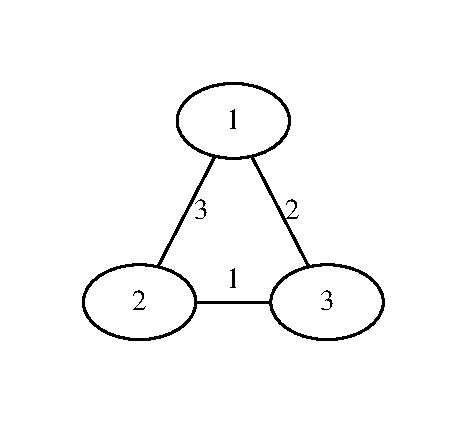
\includegraphics[width= .4\textwidth]{8-4-1.pdf}

Then, $T$ is:

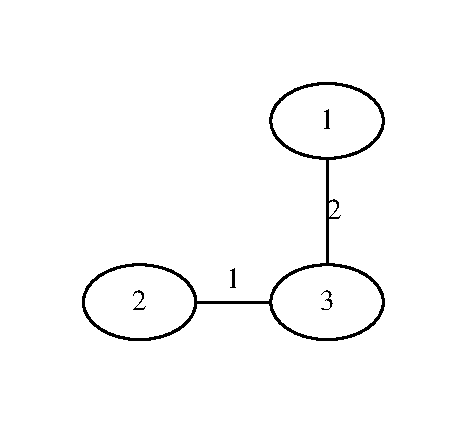
\includegraphics[width= .4\textwidth]{8-4-2.pdf}

$G_{1.5}$ is:

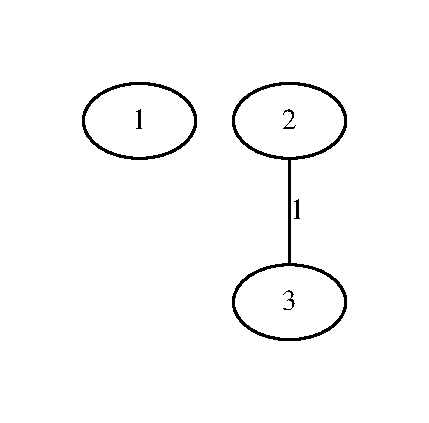
\includegraphics[width= .4\textwidth]{8-4-3.pdf}

$T_{1.5}$ is:
    
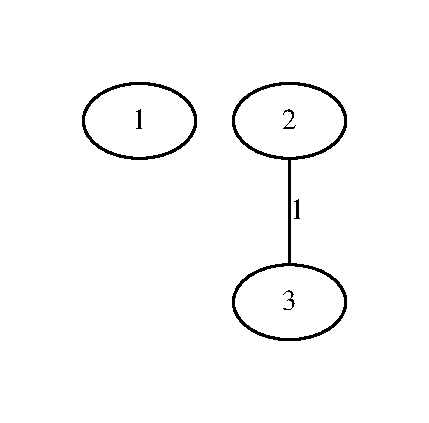
\includegraphics[width= .4\textwidth]{8-4-3.pdf}

$G_{1.5}$ and $T_{1.5}$ have the same connected components.

\begin{exercise}
     Prove the lemma.
\end{exercise}

\begin{proof}

    In \emph{Kruskal Algorithm}, $\forall c \in \R, \forall e_i$ that $w(e)\leq c$, at the step considering it, if we can put $e_k$ in $T$, then we can put it in $T_c$, which will result in $T_c$'s connected component reduced by one, and since it does not cause a cycle in $T_c$, it does not cause a cycle in $G_c$, which will reduce $G_c$'s connected components by one. If we cannot add it into $T$, obviously this edge does not affect $T_c$, and since it causes a cycle in $T$, it will not reduce the connected components when added to $G_c$. In conclusion, each edge has the same influence on $T_c$ and $G_c$ at the step selecting them.

\end{proof}

\begin{definition}
  For a weighted graph $G$, let $m_c(G) := | \{ e \in E(G) \ | \ w(e) \leq c\}|$, i.e.,
  the number of edges of weight at most $c$ (so $G_c$ has $m_c(G)$ edges).
\end{definition}

\begin{lemma}
  Let $T, T'$ be two minimum spanning trees of $G$. Then
  $m_c(T) = m_c(T')$.
  \label{lemma-weight-multiplicity}
\end{lemma}

\begin{exercise}
Illustrate Lemma~\ref{lemma-weight-multiplicity} with an example!
\end{exercise}

\textbf{Solution.}
%\par
    %$V=\{v_1,v_2\},E=\{(v_1,v_2)\}$, $T=\{(v_1,v_2)\}$. Obviously they are the same.
For example, $G$ is:

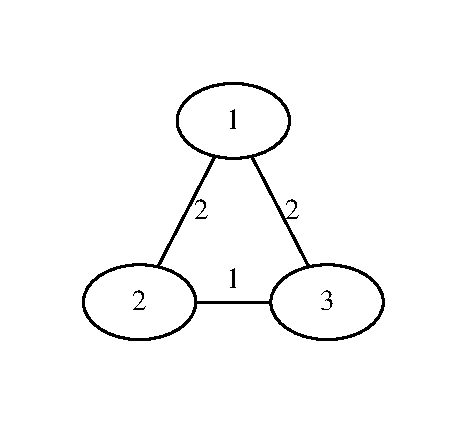
\includegraphics[width= .4\textwidth]{8-8-1.pdf}

$T$ is:

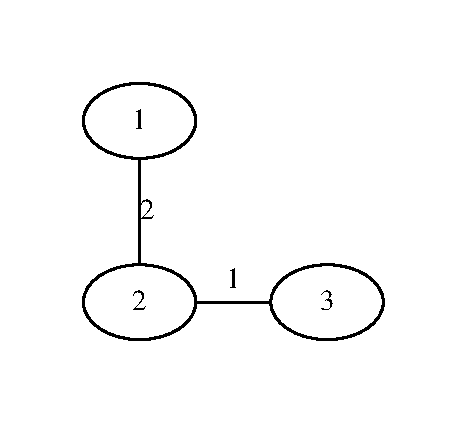
\includegraphics[width= .4\textwidth]{8-8-2.pdf}

$T^{\prime}$ is:

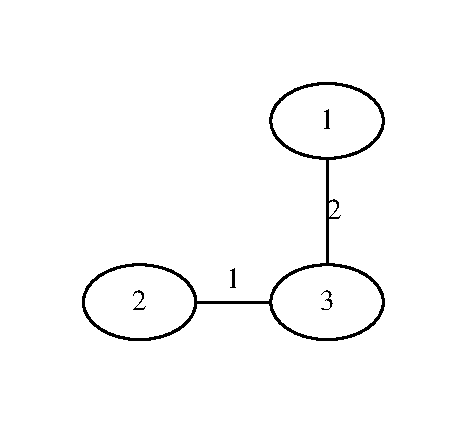
\includegraphics[width= .4\textwidth]{8-8-3.pdf}

$T_{1.5}$ is:

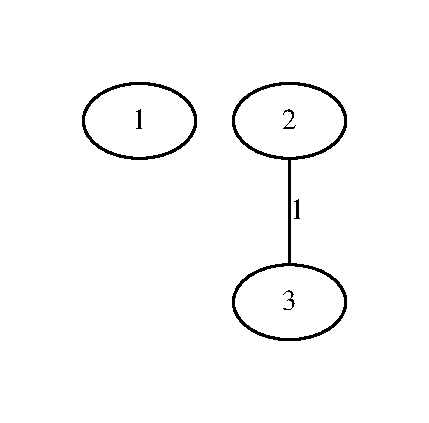
\includegraphics[width= .4\textwidth]{8-8-4.pdf}

$T_{1.5}^{\prime}$ is:

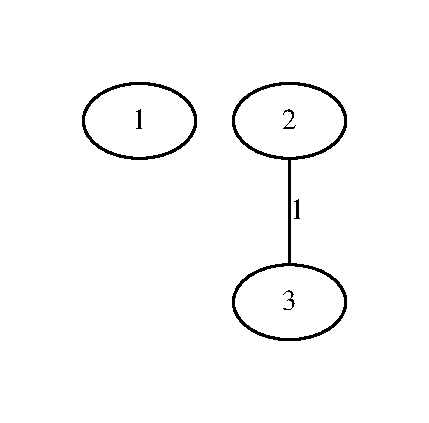
\includegraphics[width= .4\textwidth]{8-8-4.pdf}

$T_{1.5}$ and $T_{1.5}^{\prime}$ all have 1 edge.

\begin{exercise}
Prove the lemma.
\end{exercise}
\begin{proof}
$$
    \begin{aligned}
    m_c(T) & = m_{+\infty}(T_c)\\
    & = |E|-\text{connected component}(T_c)\\
    & = |E|-\text{connected component}(G_c)\\
    & = |E|-\text{connected component}(T'_c)\\
    & = m_{+\infty}(T'_c)\\
    & = m_c(T')\\
    \end{aligned}
$$
\end{proof}

\begin{exercise}
  Suppose no two edges of $G$ have the same weight.
  Show that $G$ has exactly one minimum spanning tree!
\end{exercise}

\begin{proof}
    Suppose there are two minimum spanning tree $T$ and $T^{\prime}$. Consider in \emph{Kruskal Alogorithm}, the first step where they add an edge to themselves is that $T$ chooses $e_i$ while $T^{\prime}$ chooses $e_j$. However, since they are precisely the same after the last step, $e_i$ and $e_j$ must have the same weight so that they are taken into consideration at the same time, which contradicts with the conditions.
\end{proof}


